% Work-MAT | 2. rocnik | hodina 11
\documentclass[11pt,a4paper]{article}
\input{../../sablony/pripravy/priprava.sty}
\usepackage{tikz}
\usetikzlibrary{arrows.meta}
\nastavPripravu{2. ročník}{Exponenciální funkce}{11}{Exponenciální funkce I: zavedení}
\begin{document}
\poznamka{Návaznost na hodinu 10: rozlišit $x^2$ a $2^x$. Orientačně 6 min motivace, 12 min zavedení, 9 min tabulka a graf, 12 min příklady, 6 min samostatné upevnění. Zatím bez logaritmů.}
\blok{Od mocninné k exponenciální funkci}
U mocninné funkce $x^2$ dosazujeme proměnnou za základ; exponent se nemění. Nyní budeme umocňovat stále stejné číslo, ale měnit \emph{exponent}. Pro $f(x)=2^x$ známe z pravidel pro mocniny
\[
\begin{array}{c|rrrrrr}
x&-2&-1&0&1&2&3\\\hline
x^2&4&1&0&1&4&9\\
2^x&\frac{1}{4}&\frac{1}{2}&1&2&4&8
\end{array}
\]
Z pouhých hodnot vidíme, že jde o různé funkce. Důležitý je i význam záporného exponentu: $2^{-2}=\frac{1}{2^2}$, nikoli $-4$.\par
\begin{prikladReseniBox}[title={Příklad 1}]
Co se stane, jestliže položíme $a=1$? Sestav tabulku hodnot $f(x)=1^x$ pro několik argumentů a urči druh funkce.
\tcblower
\[
\begin{array}{c|rrrrr}
x&-2&-1&0&1&2\\\hline
1^x&1&1&1&1&1
\end{array}
\]
Pro každé $x\in\mathbb R$ dostáváme $1^x=1$, takže předpis $f(x)=1$ určuje \textbf{konstantní funkci} a grafem je vodorovná přímka $y=1$. Proto číslo $1$ jako základ exponenciální funkce nepřipouštíme.
\end{prikladReseniBox}
\begin{definiceBox}[title={Definice - Exponenciální funkce}]
\textbf{Exponenciální funkce} o základu $a$ má předpis $f(x)=a^x$, kde $a>0$ a $a\ne1$; je definována pro všechna $x\in\mathbb R$. 
\end{definiceBox}
Proč vyžadujeme $a>0$? Nulu nelze umocnit například na $-1$; záporný základ nemá v reálných číslech smysl pro každý necelý exponent.\par
\begin{center}
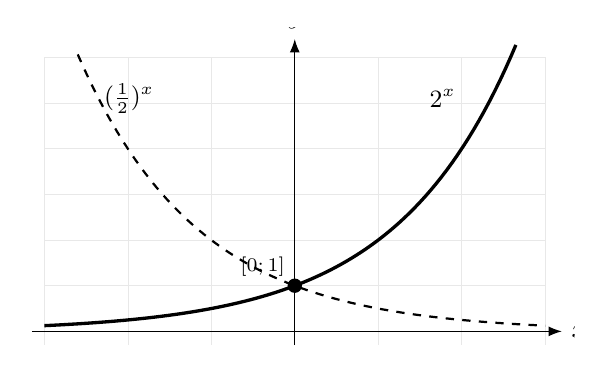
\begin{tikzpicture}[x=1.06cm,y=.58cm,>=Latex]
\clip(-3.2,-.45)rectangle(3.35,6.65);
\draw[step=1,gray!18,very thin](-3,-.3)grid(3,6);
\draw[->](-3.15,0)--(3.2,0)node[right]{$x$};
\draw[->](0,-.3)--(0,6.4)node[above]{$y$};
\draw[very thick,domain=-3:2.65,samples=90]plot(\x,{pow(2,\x)});
\draw[thick,dashed,domain=-2.6:3,samples=90]plot(\x,{pow(0.5,\x)});
\fill(0,1)circle(2.6pt);
\node[anchor=west,font=\small]at(1.5,5.1){$2^x$};
\node[anchor=west,font=\small]at(-2.4,5.1){$(\frac{1}{2})^x$};
\node[anchor=south east,font=\scriptsize]at(0,1){$[0;1]$};
\end{tikzpicture}
\end{center}
\poznamka{Plná křivka roste, čárkovaná klesá. Žáci mají výslovně říci, proč oba grafy procházejí bodem $[0;1]$ a proč nikde nedávají nulu.}
Protože $a^0=1$, prochází každá exponenciální funkce bodem $[0;1]$. Její funkční hodnoty jsou kladné, graf tedy nikdy neprotíná osu $x$; přímka $y=0$ je vodorovnou asymptotou. Zároveň platí $D(f)=\mathbb R$ a $H(f)=(0;+\infty)$.
\begin{zadaniBox}[title={Věta - Monotónnost exponenciální funkce}]
Pro $a>1$ je exponenciální funkce $f(x)=a^x$ \textbf{rostoucí}. Pro $0<a<1$ je \textbf{klesající}.
\end{zadaniBox}
\blok{Výpočty, rozpoznávání předpisů a čtení grafu}
\begin{prikladReseniBox}[title={Příklad 2}]
Pro $f(x)=3^x$ vypočti funkční hodnoty a urči monotónnost:
\begin{enumerate}[label=\alph*)]
\item $f(-2)$, $f(0)$, $f(1)$;
\item $f(2)$, $f(\frac{1}{2})$;
\item $D(f)$ a $H(f)$.
\end{enumerate}
\tcblower
\begin{enumerate}[label=\alph*)]
\item $f(-2)=\frac{1}{9}$, $f(0)=1$, $f(1)=3$.
\item $f(2)=9$, $f(\frac{1}{2})=\sqrt3$.
\item $D(f)=\mathbb R$, $H(f)=(0;+\infty)$. Funkce roste, protože $3>1$.
\end{enumerate}
\end{prikladReseniBox}
\begin{prikladReseniBox}[title={Příklad 3}]
Rozhodni, které předpisy představují exponenciální funkce, a urči jejich monotónnost:
\begin{enumerate}[label=\alph*)]
\item $f(x)=4^x$;
\item $g(x)=x^4$;
\item $h(x)=1^x$;
\item $k(x)=\left(\frac{1}{5}\right)^x$;
\item $m(x)=(-2)^x$.
\end{enumerate}
\tcblower
\begin{enumerate}[label=\alph*)]
\item Exponenciální, roste.
\item Mocninná funkce, není exponenciální.
\item Konstantní funkce $h(x)=1$, nikoli exponenciální v našem vymezení.
\item Exponenciální, klesá.
\item Předpis není definován pro všechna reálná $x$, a proto nejde o reálnou exponenciální funkci.
\end{enumerate}
\end{prikladReseniBox}
\begin{prikladReseniBox}[title={Příklad 4}]
Sestav předpis základní exponenciální funkce $f(x)=a^x$:
\begin{enumerate}[label=\alph*)]
\item $f(1)=5$;
\item $f(-1)=4$.
\end{enumerate}
U obou načrtni graf a vyznač bod $[0;1]$.
\tcblower
\begin{enumerate}[label=\alph*)]
\item $a^1=5$, tedy $f(x)=5^x$ (rostoucí).
\item $a^{-1}=4$, tedy $\frac{1}{a}=4$, $a=\frac{1}{4}$ a $f(x)=\left(\frac{1}{4}\right)^x$ (klesající).
\end{enumerate}
Oba grafy procházejí bodem $[0;1]$ a mají asymptotu $y=0$.
\end{prikladReseniBox}
\begin{prikladReseniBox}[title={Příklad 5}]
Urči předpis základní exponenciální funkce $f(x)=a^x$ a její monotónnost:
\begin{enumerate}[label=\alph*)]
\item $f(2)=16$;
\item $f(-2)=9$;
\item $f(3)=\frac{1}{8}$.
\end{enumerate}
\tcblower
\begin{enumerate}[label=\alph*)]
\item $a^2=16$, $a>0$, tedy $a=4$ a $f(x)=4^x$ (roste).
\item $a^{-2}=9$, tedy $a^2=\frac{1}{9}$, $a=\frac{1}{3}$ a $f(x)=\left(\frac{1}{3}\right)^x$ (klesá).
\item $a^3=\frac{1}{8}$, tedy $a=\frac{1}{2}$ a $f(x)=\left(\frac{1}{2}\right)^x$ (klesá).
\end{enumerate}
\end{prikladReseniBox}
\begin{zadaniReseniBox}[title={Samostatná práce 1}]
\begin{enumerate}[label=\alph*)]
\item $2^{-2}$, $2^0$, $2^3$: vypočti a sestav tabulku pro $f(x)=2^x$.
\item U $g(x)=\left(\frac{1}{3}\right)^x$ vypočti $g(-2)$, $g(1)$, $g(2)$.
\item Která funkce roste: $4^x$, nebo $\left(\frac{1}{4}\right)^x$? Proč?
\item Rozhodni, zda $x^5$ a $5^x$ představují stejný typ funkce.
\item Sestav $a^x$ z hodnoty $f(1)=\frac{1}{6}$.
\item Sestav $a^x$ z hodnoty $f(2)=49$.
\item Který graf má s osou $x$ společný bod: $3^x$, nebo $x^3$?
\item Načrtni graf $y=\left(\frac{1}{2}\right)^x$ a označ alespoň čtyři body.
\end{enumerate}
\tcblower
\begin{enumerate}[label=\alph*)]
\item $\frac{1}{4}$, $1$, $8$.
\item $9$, $\frac{1}{3}$, $\frac{1}{9}$.
\item $4^x$ roste; druhá funkce klesá.
\item $x^5$ mocninná, $5^x$ exponenciální.
\item $\left(\frac{1}{6}\right)^x$.
\item $7^x$.
\item $x^3$ má nulový bod $x=0$; $3^x>0$.
\item Například $[-2;4]$, $[-1;2]$, $[0;1]$, $[1;\frac{1}{2}]$.
\end{enumerate}
\end{zadaniReseniBox}
\begin{zadaniReseniBox}[title={Rozšíření 1}]
\begin{enumerate}[label=\alph*)]
\item Exponenciální funkce $f(x)=a^x$ splňuje $\frac{f(x+2)}{f(x)}=25$ pro libovolné $x$. Urči základ $a$ a monotónnost.
\item Vysvětli, proč tato podmínka nezávisí na konkrétním $x$.
\end{enumerate}
\tcblower
\begin{enumerate}[label=\alph*)]
\item $\frac{a^{x+2}}{a^x}=a^2=25$ a $a>0$, tedy $a=5$; funkce roste.
\item Při posunu exponentu o dvě se hodnota vždy násobí stejným číslem $a^2$.
\end{enumerate}
\end{zadaniReseniBox}
\clearpage
\begin{zadaniReseniBox}[title={Domácí úkol}]
\begin{enumerate}[label=\alph*)]
\item Urči $D$, $H$, monotónnost a průsečík s osou $y$ pro $2^x$.
\item Totéž proveď pro $\left(\frac{1}{3}\right)^x$.
\item Vypočti $2^{-3}$, $4^{\frac{1}{2}}$, $9^{-\frac{1}{2}}$.
\item Vysvětli rozdíl mezi $x^3$ a $3^x$.
\item Rozhodni, zda je $\left(\frac{5}{4}\right)^x$ rostoucí, či klesající.
\item Sestav $f(x)=a^x$, jestliže $f(1)=7$.
\item Sestav $g(x)=a^x$, jestliže $g(-1)=5$.
\item Sestav $h(x)=a^x$, jestliže $h(2)=\frac{1}{16}$.
\item V jedné soustavě souřadnic načrtni $2^x$ a $\left(\frac{1}{2}\right)^x$; vyznač nejméně čtyři body každé křivky.
\item Vysvětli, proč $1^x$ není exponenciální funkcí podle zavedené definice.
\end{enumerate}
\tcblower
\begin{enumerate}[label=\alph*)]
\item $D=\mathbb R$, $H=(0;+\infty)$; roste, $[0;1]$.
\item $D=\mathbb R$, $H=(0;+\infty)$; klesá, $[0;1]$.
\item $\frac{1}{8}$, $2$, $\frac{1}{3}$.
\item V $x^3$ se mění základ; v $3^x$ exponent.
\item Roste, protože $\frac{5}{4}>1$.
\item $f(x)=7^x$.
\item $g(x)=\left(\frac{1}{5}\right)^x$.
\item $h(x)=\left(\frac{1}{4}\right)^x$.
\item Pro $2^x$: $[-2;\frac{1}{4}]$, $[-1;\frac{1}{2}]$, $[0;1]$, $[1;2]$. Druhý graf: $[-1;2]$, $[0;1]$, $[1;\frac{1}{2}]$, $[2;\frac{1}{4}]$.
\item Při $a=1$ je $f(x)=1$, tedy konstantní funkce.
\end{enumerate}
\end{zadaniReseniBox}
\poznamka{Domácí úkol: zhruba 20--25 minut; ve třídě lze zadat jen vybrané podúlohy. Grafy nechat skutečně sestrojit do sešitu.}
\end{document}
